\documentclass{article}
\usepackage{amssymb,fullpage,listings,url} 

\usepackage{graphicx} % Required for inserting images

\newtheorem{theorem}{Theorem}
\newtheorem{property}{Property}

\def\st{{\ :\ }}
\def\bbR{\mathbb{R}}
\def\bbD{\mathbb{D}}
\def\bbC{\mathbb{C}}
\def\inner#1#2{\langle #1,#2\rangle}

\title{Reflection about a geodesic passing through two given points in the Poincar\'e and Klein disk  models of hyperbolic geometry}

\author{Frank Nielsen\\ Sony Computer Science Laboratories Inc\\ Tokyo }

\date{15 December 2023}

\begin{document}

\maketitle

\begin{abstract}
We report in this note a direct closed-form formula for the reflection operation about a geodesic defined by two given points  in the Poincar\'e disk.
\end{abstract}

\section{Geodesics and pregeodesics}

In metric geometry (including Riemannian geometry) with distance $\rho$, a geodesic $\gamma(l)$ is parameterized by a constant speed parameter $l$ so that we have 
$$
\rho(\gamma(l),\gamma(l'))=|l-l'|\, \rho(\gamma(0),\gamma(1)).
$$
The constant speed parameterization is related to arc length parameterization by $s=l\,\rho(\gamma(0),\gamma(1))$, where $p_0=\gamma(0)$ and $p_1=\gamma(1)$ are the geodesic endpoints.

To constrast with geodesics, a pregeodesic $\bar\gamma(t)=\bar\gamma(l(t))$ is a reparameterization of the geodesic such that $l(t)$ is a smooth and invertible with inverse function $t(l)$. Pregeodesics can yield simplified mathematical expressions of parameterizations, and express equivalently the geodesic curves:
$$
c_\gamma=\{\gamma(l) \st l\in [0,1]\} = \{\bar\gamma(t) \st t\in [a,b]\}.
$$

For example, in the Klein model of hyperbolic geometry, pregeodesics passing through two given points $k_1$ and $k_2$ of the unit disk $\bbD$ are Euclidean line segments parameterized by:
$$
\bar\gamma_K(t)=k_1+t(k_2-k_1),
$$
with geodesic curve $c_{\gamma_K}=[k_1k_2]$.
The geodesic equation with constant speed parameterization in Klein model has been reported in~\cite{nielsen2012hyperbolic}, i.e., the function $l(t)$ such that
$$
\gamma_K(l)=\bar\gamma_K(l(t))
$$
is given in closed-form.

\section{Geodesic curves in Klein model}

To find the complete geodesic $\Gamma_K=\{\gamma_K(l) \st l\in\bbR\}$ in Klein model, we need to find $t_m$ and $t_M$ such that $\Gamma_K$ is the line passing through $[k_1k_2]$ clipped to the unit disk $\bbD$.
$t_m$ and $t_M$ are the two solutions of the quadratic equation:
$$
\inner{k_1+t(k_2-k_1)}{k_1+t(k_2-k_1)}=1
$$

A model of a geometry is said conformal if the angles of two curves $c_1(t)$ and $c_2(t)$ intersecting at $t_0$ match the Euclidean angles.
The Poincar\'e disk model is conformal but not the Klein model (except at the origin).

\def\reflect{\mathrm{reflect}}
%%%
\section{Reflections about geodesics in the Poincar\'e disk model}
%%%%

Geodesics in the Poincar\'e model  are either arc of circles perpendicular to the disk boundary $\partial\bbD$, or line segments passing through the origin.
Poincar\'e geodesic curves are sometimes called clines~\cite{hitchman2009geometry} (circles or lines).
The isometries in the  Poincar\'e model seen as a subset of the complex plane $\bbC$ are M\"obius transformations.
In particular, reflections around a complete geodesic curve $\Gamma_{z_1z_2}$ passing through two given points $z_1, z_2\in\bbD$ is an Euclidean circle inversion, and thus defined by
$$
\reflect(z)=\frac{r_0^2}{\bar{z}-\bar{z}_0}+z_0.
$$


For example, such reflection operations are used for embeddings tree structures into the Poincar\'e disk~\cite{sala2018representation}.
Usually, reflections are implemented via translations to the origin of the disk. We report in this note a direct closed-form formula.


The reflection leaves the geodesic $\Gamma_{z_1z_2}$ invariant:
$$
\forall z\in \Gamma_{z_1z_2}, \reflect(z)=z,
$$
and we have $\reflect(\reflect(z))=z$ for any $z\in\bbD$.

\begin{figure}
\begin{center}
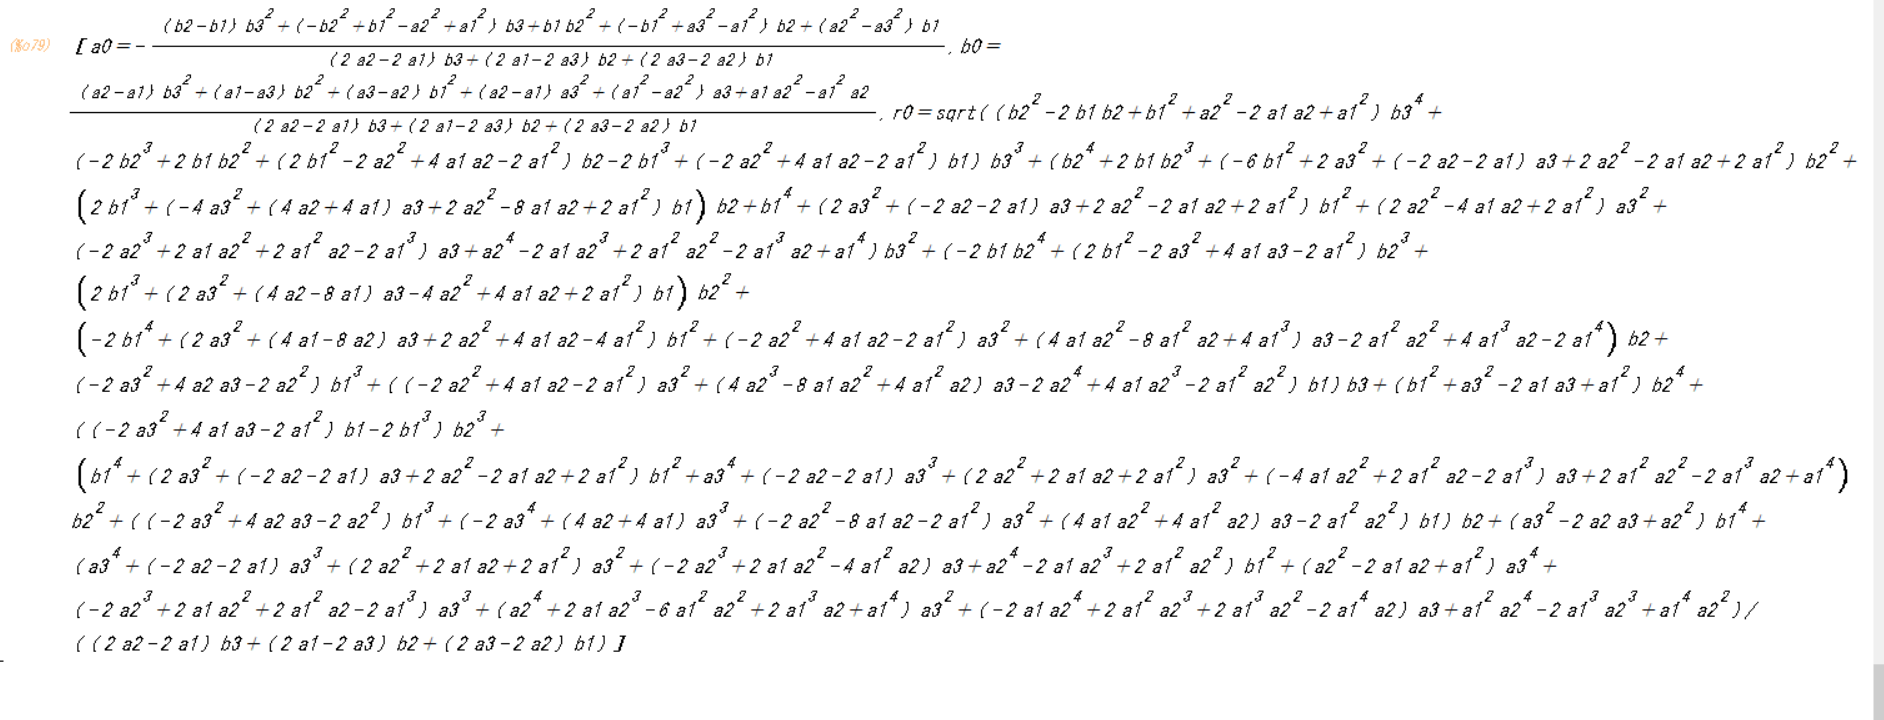
\includegraphics[width=\textwidth]{ReflectionPoincare3Points.png}
 \end{center}
\caption{Solution of the systems of equation defined in Eq.~\ref{eq:syst}.\label{fig:solve} }
\end{figure}

Let $z_3\in\Gamma_{z_1z_2}$ be any point inside the Poincar\'e geodesic.
For example, we consider $k_3$ the Klein interior point given by $\frac{k_1+k_2}{2}$ where
$$
k_i= \frac{2}{1+z_i\bar z_i}\, z_i,\quad i\in\{1,2\},
$$
and we convert the Klein geodesic interior point to the Poincar\'e disk:
$$
z_3=\frac{1-\sqrt{1-\|k_3\|^2}}{\|k_3\|^2} \, k_3
$$

Then we write the system of equations with $z_j=a_j+ib_j$ for $j\in\{0,1,2,3\}$:
\begin{equation}
\left\{
\begin{array}{lll}
\reflect(a_1+ib_1) &=& a_1+ib_1,\\
\reflect(a_2+ib_2) &=& a_2+ib_2,\\
\reflect(a_3+ib_3) &=& a_3+ib_3.
\end{array}
\right. \label{eq:syst}
\end{equation}



\begin{figure}
\centering
\begin{tabular}{cc}
Poincar\'e disk & Klein disk\\ \hline
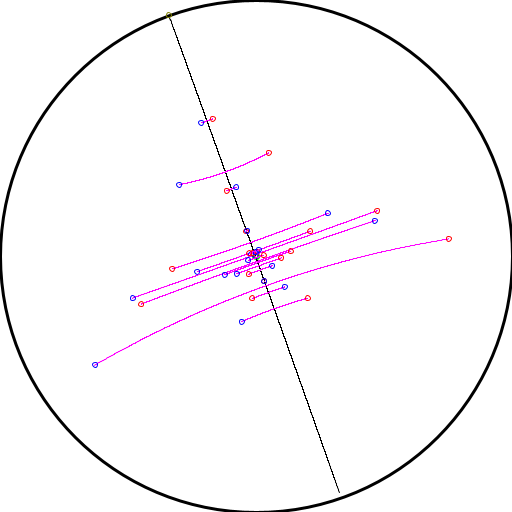
\includegraphics[width=0.3\textwidth]{PoincareReflectionGeodesics-1.png} &
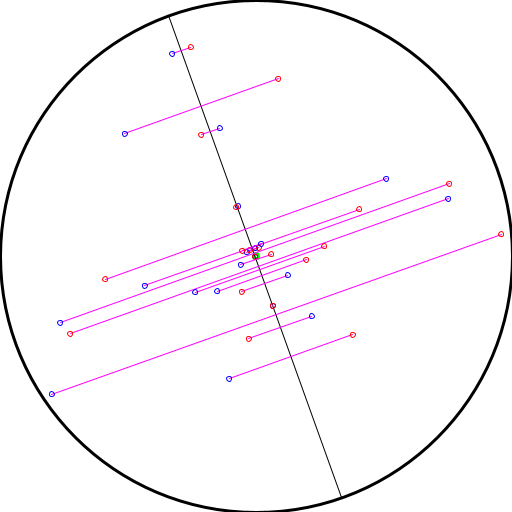
\includegraphics[width=0.3\textwidth]{KleinReflectionGeodesics-1.png} \\
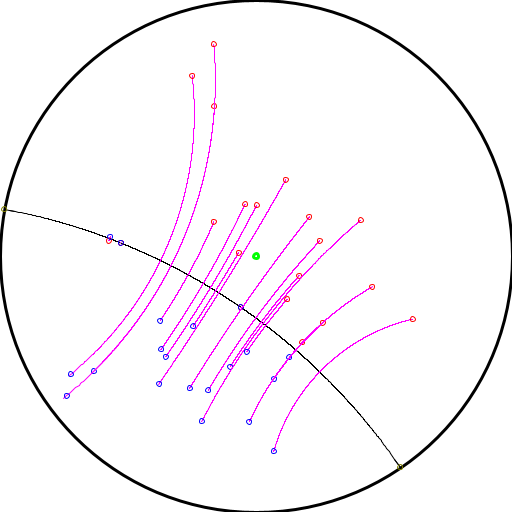
\includegraphics[width=0.3\textwidth]{PoincareReflectionGeodesics-2.png} &
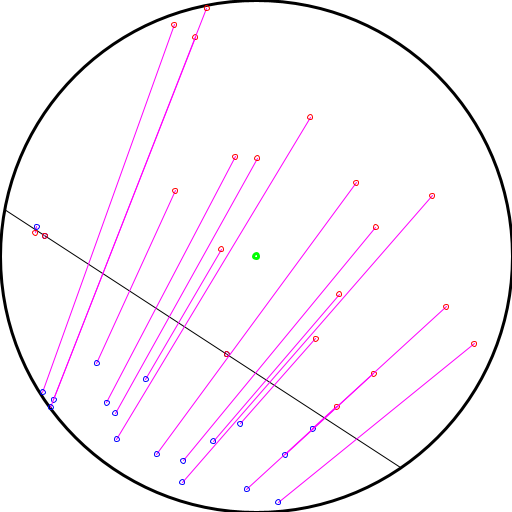
\includegraphics[width=0.3\textwidth]{KleinReflectionGeodesics-2.png} 
 \end{tabular}
\caption{Illustrating reflections around geodesics on the Poincar\'e and Klein disks.}\label{fig:illustration}
\end{figure}

Next, we use the computer algebra system {\tt Maxima}\footnote{\url{https://maxima.sourceforge.io/}} to solve the system of Eq.~\ref{eq:syst} (Figure~\ref{fig:solve}) using the code:

{\tiny
\begin{lstlisting}
z1:a1+b1*%i;
z2:a2+b2*%i;
z3:a3+b3*%i;

/* circle inversion */
reflect(z,a0,b0,r0):=(r0**2/(conjugate(z)-conjugate(a0+b0*%i)))+a0+b0*%i;

/* reflection of the points z1, z2, z3 should be identity */
reflect(z1,a0,b0,r0);
realpart(%);ratsimp(%);
eq1: %=a1;
reflect(z1,a0,b0,r0);
imagpart(%);ratsimp(%);
eq2: %=b1;
 reflect(z2,a0,b0,r0);
realpart(%);ratsimp(%);
eq3: %=a2;
reflect(z2,a0,b0,r0);
imagpart(%);ratsimp(%);
eq4: %=b2;
 reflect(z3,a0,b0,r0);
realpart(%);ratsimp(%);
eq5: %=a3;
reflect(z3,a0,b0,r0);
imagpart(%);ratsimp(%);
eq6: %=b3;

solve([eq1,eq2,eq3,eq4,eq5,eq6],[a0,b0,r0]);
solution: %[2];
\end{lstlisting}
}

{\tt Maxima} reports the unique solution for $z_0=a_0+ib_0$ and $r_0$ defining the reflection:

$$
a_{0}=-{{\left(b_{2}-b_{1}\right)\,b_{3}^2+\left(-b_{2}^2+b_{1}^2-
 a_{2}^2+a_{1}^2\right)\,b_{3}+b_{1}\,b_{2}^2+\left(-b_{1}^2+a_{3}^2-
 a_{1}^2\right)\,b_{2}+\left(a_{2}^2-a_{3}^2\right)\,b_{1}}\over{
 \left(2\,a_{2}-2\,a_{1}\right)\,b_{3}+\left(2\,a_{1}-2\,a_{3}\right)
 \,b_{2}+\left(2\,a_{3}-2\,a_{2}\right)\,b_{1}}}
$$


$$b_{0}={{\left(a_{2}-a_{1}\right)\,b_{3}^2+\left(a_{1}-a_{3}\right)
 \,b_{2}^2+\left(a_{3}-a_{2}\right)\,b_{1}^2+\left(a_{2}-a_{1}\right)
 \,a_{3}^2+\left(a_{1}^2-a_{2}^2\right)\,a_{3}+a_{1}\,a_{2}^2-a_{1}^2
 \,a_{2}}\over{\left(2\,a_{2}-2\,a_{1}\right)\,b_{3}+\left(2\,a_{1}-2
 \,a_{3}\right)\,b_{2}+\left(2\,a_{3}-2\,a_{2}\right)\,b_{1}}}$$

Parameter $r_0$ has a complex expression reported in the screenshot~\ref{fig:solve}.

%$$r_{0}={{\sqrt{\left(b_{2}^2-2\,b_{1}\,b_{2}+b_{1}^2+a_{2}^2-2\,
 %a_{1}\,a_{2}+a_{1}^2\right)\,b_{3}^4+\left(-2\,b_{2}^3+2\,b_{1}\,
 %b_{2}^2+\left(2\,b_{1}^2-2\,a_{2}^2+4\,a_{1}\,a_{2}-2\,a_{1}^2
 %\right)\,b_{2}-2\,b_{1}^3+\left(-2\,a_{2}^2+4\,a_{1}\,a_{2}-2\,a_{1}
 %^2\right)\,b_{1}\right)\,b_{3}^3+\left(b_{2}^4+2\,b_{1}\,b_{2}^3+
 %\left(-6\,b_{1}^2+2\,a_{3}^2+\left(-2\,a_{2}-2\,a_{1}\right)\,a_{3}+
 %2\,a_{2}^2-2\,a_{1}\,a_{2}+2\,a_{1}^2\right)\,b_{2}^2+\left(2\,b_{1}
 %^3+\left(-4\,a_{3}^2+\left(4\,a_{2}+4\,a_{1}\right)\,a_{3}+2\,a_{2}^
 %2-8\,a_{1}\,a_{2}+2\,a_{1}^2\right)\,b_{1}\right)\,b_{2}+b_{1}^4+
 %\left(2\,a_{3}^2+\left(-2\,a_{2}-2\,a_{1}\right)\,a_{3}+2\,a_{2}^2-2
 %\,a_{1}\,a_{2}+2\,a_{1}^2\right)\,b_{1}^2+\left(2\,a_{2}^2-4\,a_{1}
 %\,a_{2}+2\,a_{1}^2\right)\,a_{3}^2+\left(-2\,a_{2}^3+2\,a_{1}\,a_{2}
 %^2+2\,a_{1}^2\,a_{2}-2\,a_{1}^3\right)\,a_{3}+a_{2}^4-2\,a_{1}\,
 %a_{2}^3+2\,a_{1}^2\,a_{2}^2-2\,a_{1}^3\,a_{2}+a_{1}^4\right)\,b_{3}^
 %2+\left(-2\,b_{1}\,b_{2}^4+\left(2\,b_{1}^2-2\,a_{3}^2+4\,a_{1}\,
 %a_{3}-2\,a_{1}^2\right)\,b_{2}^3+\left(2\,b_{1}^3+\left(2\,a_{3}^2+
 %\left(4\,a_{2}-8\,a_{1}\right)\,a_{3}-4\,a_{2}^2+4\,a_{1}\,a_{2}+2\,
 %a_{1}^2\right)\,b_{1}\right)\,b_{2}^2+\left(-2\,b_{1}^4+\left(2\,
 %a_{3}^2+\left(4\,a_{1}-8\,a_{2}\right)\,a_{3}+2\,a_{2}^2+4\,a_{1}\,
 %a_{2}-4\,a_{1}^2\right)\,b_{1}^2+\left(-2\,a_{2}^2+4\,a_{1}\,a_{2}-2
 %\,a_{1}^2\right)\,a_{3}^2+\left(4\,a_{1}\,a_{2}^2-8\,a_{1}^2\,a_{2}+
 %4\,a_{1}^3\right)\,a_{3}-2\,a_{1}^2\,a_{2}^2+4\,a_{1}^3\,a_{2}-2\,
 %a_{1}^4\right)\,b_{2}+\left(-2\,a_{3}^2+4\,a_{2}\,a_{3}-2\,a_{2}^2
 %\right)\,b_{1}^3+\left(\left(-2\,a_{2}^2+4\,a_{1}\,a_{2}-2\,a_{1}^2
 %\right)\,a_{3}^2+\left(4\,a_{2}^3-8\,a_{1}\,a_{2}^2+4\,a_{1}^2\,
 %a_{2}\right)\,a_{3}-2\,a_{2}^4+4\,a_{1}\,a_{2}^3-2\,a_{1}^2\,a_{2}^2
 %\right)\,b_{1}\right)\,b_{3}+\left(b_{1}^2+a_{3}^2-2\,a_{1}\,a_{3}+
 %a_{1}^2\right)\,b_{2}^4+\left(\left(-2\,a_{3}^2+4\,a_{1}\,a_{3}-2\,
 %a_{1}^2\right)\,b_{1}-2\,b_{1}^3\right)\,b_{2}^3+\left(b_{1}^4+
 %\left(2\,a_{3}^2+\left(-2\,a_{2}-2\,a_{1}\right)\,a_{3}+2\,a_{2}^2-2
 %\,a_{1}\,a_{2}+2\,a_{1}^2\right)\,b_{1}^2+a_{3}^4+\left(-2\,a_{2}-2
 %\,a_{1}\right)\,a_{3}^3+\left(2\,a_{2}^2+2\,a_{1}\,a_{2}+2\,a_{1}^2
 %\right)\,a_{3}^2+\left(-4\,a_{1}\,a_{2}^2+2\,a_{1}^2\,a_{2}-2\,a_{1}
 %^3\right)\,a_{3}+2\,a_{1}^2\,a_{2}^2-2\,a_{1}^3\,a_{2}+a_{1}^4
 %\right)\,b_{2}^2+\left(\left(-2\,a_{3}^2+4\,a_{2}\,a_{3}-2\,a_{2}^2
 %\right)\,b_{1}^3+\left(-2\,a_{3}^4+\left(4\,a_{2}+4\,a_{1}\right)\,
 %a_{3}^3+\left(-2\,a_{2}^2-8\,a_{1}\,a_{2}-2\,a_{1}^2\right)\,a_{3}^2
 %+\left(4\,a_{1}\,a_{2}^2+4\,a_{1}^2\,a_{2}\right)\,a_{3}-2\,a_{1}^2
 %\,a_{2}^2\right)\,b_{1}\right)\,b_{2}+\left(a_{3}^2-2\,a_{2}\,a_{3}+
 %a_{2}^2\right)\,b_{1}^4+\left(a_{3}^4+\left(-2\,a_{2}-2\,a_{1}
 %\right)\,a_{3}^3+\left(2\,a_{2}^2+2\,a_{1}\,a_{2}+2\,a_{1}^2\right)
 %\,a_{3}^2+\left(-2\,a_{2}^3+2\,a_{1}\,a_{2}^2-4\,a_{1}^2\,a_{2}
 %\right)\,a_{3}+a_{2}^4-2\,a_{1}\,a_{2}^3+2\,a_{1}^2\,a_{2}^2\right)
 %\,b_{1}^2+\left(a_{2}^2-2\,a_{1}\,a_{2}+a_{1}^2\right)\,a_{3}^4+
 %\left(-2\,a_{2}^3+2\,a_{1}\,a_{2}^2+2\,a_{1}^2\,a_{2}-2\,a_{1}^3
 %\right)\,a_{3}^3+\left(a_{2}^4+2\,a_{1}\,a_{2}^3-6\,a_{1}^2\,a_{2}^2
 %+2\,a_{1}^3\,a_{2}+a_{1}^4\right)\,a_{3}^2+\left(-2\,a_{1}\,a_{2}^4+
 %2\,a_{1}^2\,a_{2}^3+2\,a_{1}^3\,a_{2}^2-2\,a_{1}^4\,a_{2}\right)\,
 %a_{3}+a_{1}^2\,a_{2}^4-2\,a_{1}^3\,a_{2}^3+a_{1}^4\,a_{2}^2}}\over{
 %\left(2\,a_{2}-2\,a_{1}\right)\,b_{3}+\left(2\,a_{1}-2\,a_{3}\right)
 %\,b_{2}+\left(2\,a_{3}-2\,a_{2}\right)\,b_{1}}}$$





A point $z=a+ib$ is reflected to a point $z'=a'+ib'$ with
\begin{eqnarray*}
a' &=& \frac{(a-a_0)r_0^2}{(b_0-b)^2+(a-a_0)^2)}+a_0,\\
b' &=& \frac{(b-b_0)r_0^2}{(b_0-b)^2+(a-a_0)^2)}+b_0.
\end{eqnarray*}

 Figure~\ref{fig:illustration} illustrates some examples of reflections obtained in the Poincar\'e disk and then converted into the Klein disk.


Notice that the equation of a circle  of center $(x_0,y_0)$ and radius $r_0>0$ passing through three given points $(x_1,y_1), (x_2,y_2)$ and $(x_3,y3)$ can be found also by symbolic computing:

\begin{lstlisting}
/* equation of a circle with center (x0,y0) and radius r0 passing through 3 points (xi, yi) for i=1,2,3*/
assume(r0>0);

eq1: (x1-x0)**2 + (y1-y0)**2=  r0**2;
eq2: (x2-x0)**2 + (y2-y0)**2 = r0**2;
eq3: (x3-x0)**2 + (y3-y0)**2 = r0**2;

solve([eq1,eq2,eq3],[x0,y0,r0]);
%[2];
\end{lstlisting} 

See Figure~\ref{fig:circle3pts} for a screenshot of {\sc Maxima} result.
One way to geometrically derive this equation is to consider the unique intersection of two line bisectors defined by the three points $\{(x_i,y_i), i\in\{1,2,3\}\}$, and then calculate the radius $r_0$ as the distance of the circumcenter to the given points~\cite{nielsen2005visual}.


\begin{figure}
\centering
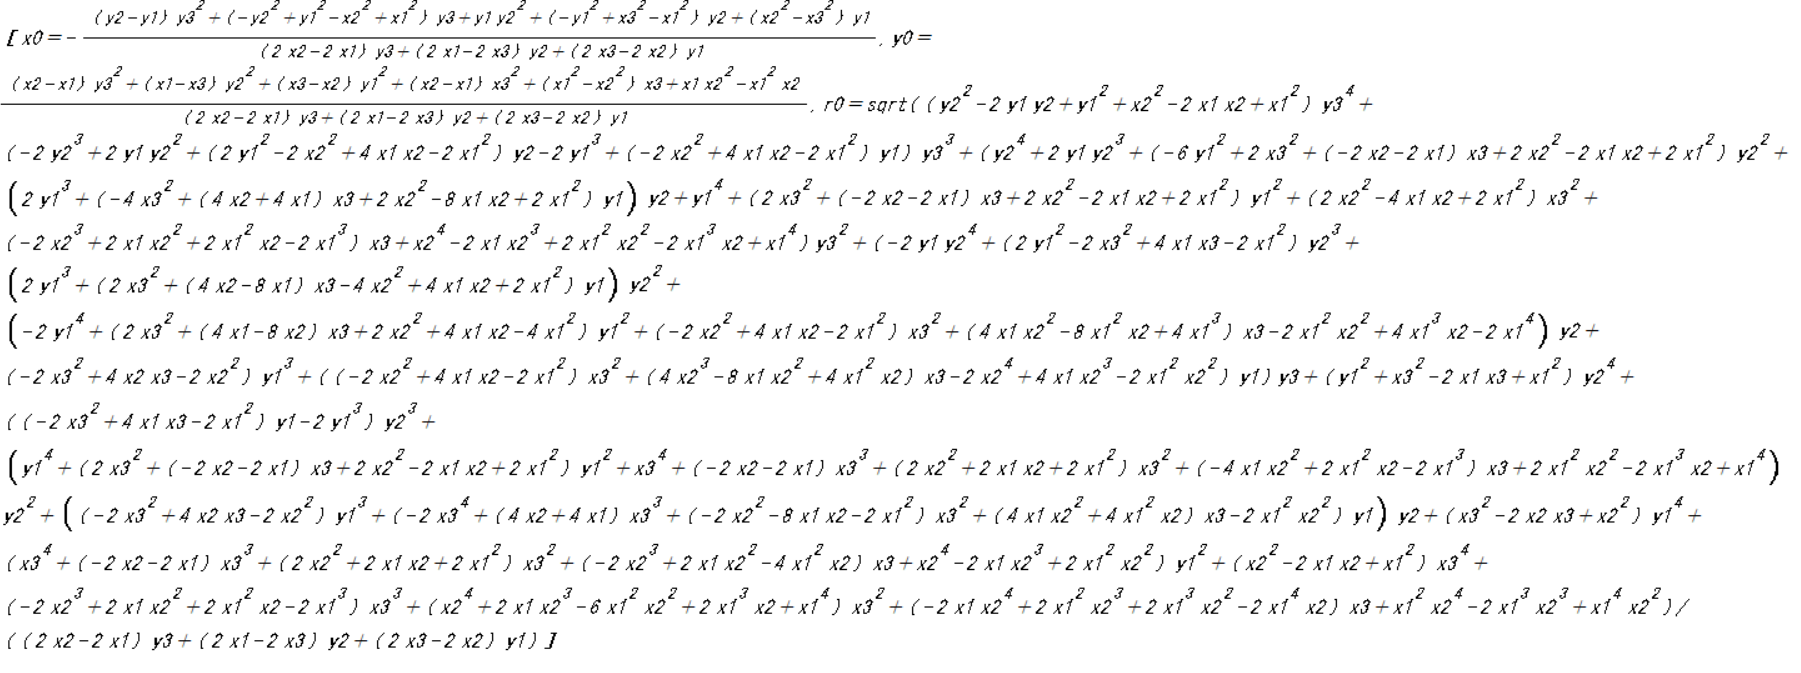
\includegraphics[width=\textwidth]{Circle3PointsEquation.png} 
\caption{Equation of a circle passing through three given points.\label{fig:circle3pts} }
\end{figure}



It is usually easy and numerically robust to implement geometric algorithms like the Voronoi diagram~\cite{nielsen2010hyperbolic} in the Klein disk and visualize the result in the conformal Poincar\'e disk.
The Poincar\'e disk may be directly considered for some problems like calculating the smallest enclosing hyperbolic ball since a hyperbolic ball in the Poincar\'e disk model is a Euclidean ball with a shifted center~\cite{tanuma2010revisiting}.

{\tiny
\begin{lstlisting}[language = Java,breaklines = true]
class Reflection
{
  double a0, b0, r0;

  public static double sqr(double x) {return x*x;}

// Reflect a point
  Point2D reflect(Point2D p)
  {
    double a=p.x; double b=p.y; double xx, yy;
    xx=      ((a-a0)*sqr(r0))/(sqr(b0-b)+sqr(a-a0))+a0;
    yy=      ((b-b0)*sqr(r0))/(sqr(b0-b)+sqr(a-a0))+b0;

    return new Point2D(xx, yy);
  }

  Reflection(double a, double b, double r)
  {
    a0=a; b0=b;r0=r;
  }

// Given three points on a Poincare geodesic (usually p3 is interior point on p1 p) calculates the coefficients of the circle inversion 
// which gives the hyperbolic reflection
  Reflection(Point2D p1, Point2D p2, Point2D p3)
  {
    double a1, b1, a2, b2, a3, b3;
    a1=p1.x;
    b1=p1.y;
    a2=p2.x;
    b2=p2.y;
    a3=p3.x;
    b3=p3.y;

    a0 = -((b2-b1)*Math.pow(b3, 2)+((-Math.pow(b2, 2))+Math.pow(b1, 2)-Math.pow(a2, 2)+Math.pow(a1, 2))*b3+b1*Math.pow(b2, 2)+((-Math.pow(b1, 2))+Math.pow(a3, 2)-Math.pow(a1, 2))*b2+(Math.pow(a2, 2)-Math.pow(a3, 2))*b1)/((2*a2-2*a1)*b3
      +(2*a1-2*a3)*b2+(2*a3-2*a2)*b1);

    b0 = ((a2-a1)*Math.pow(b3, 2)+(a1-a3)*Math.pow(b2, 2)+(a3-a2)*Math.pow(b1, 2)+(a2-a1)*Math.pow(a3, 2)+(Math.pow(a1, 2)
      -Math.pow(a2, 2))*a3+a1*Math.pow(a2, 2)-Math.pow(a1, 2)*a2)/((2*a2-2*a1)*b3+(2*a1-2*a3)*b2+(2*a3-2*a2)*b1);

    r0 = Math.sqrt((Math.pow(b2, 2)-2*b1*b2+Math.pow(b1, 2)+Math.pow(a2, 2)-2*a1*a2+Math.pow(a1, 2))*Math.pow(b3, 4)+
      ((-2*Math.pow(b2, 3))+2*b1*Math.pow(b2, 2)+(2*Math.pow(b1, 2)-2*Math.pow(a2, 2)+4*a1*a2-2*Math.pow(a1, 2))*b2
      -2*Math.pow(b1, 3)+((-2*Math.pow(a2, 2))+4*a1*a2-2*Math.pow(a1, 2))*b1)*Math.pow(b3, 3)+(Math.pow(b2, 4)+2*b1*Math.pow(b2, 3)
      +((-6*Math.pow(b1, 2))+2*Math.pow(a3, 2)+((-2*a2)-2*a1)*a3+2*Math.pow(a2, 2)-2*a1*a2+2*Math.pow(a1, 2))*Math.pow(b2, 2)
      +(2*Math.pow(b1, 3)+((-4*Math.pow(a3, 2))+(4*a2+4*a1)*a3+2*Math.pow(a2, 2)-8*a1*a2+2*Math.pow(a1, 2))*b1)*b2+Math.pow(b1, 4)
      +(2*Math.pow(a3, 2)+((-2*a2)-2*a1)*a3+2*Math.pow(a2, 2)-2*a1*a2+2*Math.pow(a1, 2))*Math.pow(b1, 2)+(2*Math.pow(a2, 2)-4*a1*a2+2*Math.pow(a1, 2))*Math.pow(a3, 2)
      +((-2*Math.pow(a2, 3))+2*a1*Math.pow(a2, 2)+2*Math.pow(a1, 2)*a2-2*Math.pow(a1, 3))*a3
      +Math.pow(a2, 4)-2*a1*Math.pow(a2, 3)+2*Math.pow(a1, 2)*Math.pow(a2, 2)-2*Math.pow(a1, 3)*a2+Math.pow(a1, 4))*Math.pow(b3, 2)+
      ((-2*b1*Math.pow(b2, 4))+(2*Math.pow(b1, 2)-2*Math.pow(a3, 2)+4*a1*a3-2*Math.pow(a1, 2))*Math.pow(b2, 3)+(2*Math.pow(b1, 3)
      +(2*Math.pow(a3, 2)+(4*a2-8*a1)*a3-4*Math.pow(a2, 2)+4*a1*a2+2*Math.pow(a1, 2))*b1)*Math.pow(b2, 2)
      +((-2*Math.pow(b1, 4))+(2*Math.pow(a3, 2)+(4*a1-8*a2)*a3+2*Math.pow(a2, 2)+4*a1*a2-4*Math.pow(a1, 2))*Math.pow(b1, 2)+((-2*Math.pow(a2, 2))+4*a1*a2-2*Math.pow(a1, 2))*Math.pow(a3, 2)
      +(4*a1*Math.pow(a2, 2)-8*Math.pow(a1, 2)*a2+4*Math.pow(a1, 3))*a3-2*Math.pow(a1, 2)*Math.pow(a2, 2)+4*Math.pow(a1, 3)*a2-2*Math.pow(a1, 4))*b2
      +((-2*Math.pow(a3, 2))+4*a2*a3-2*Math.pow(a2, 2))*Math.pow(b1, 3)+(((-2*Math.pow(a2, 2))+4*a1*a2-2*Math.pow(a1, 2))*Math.pow(a3, 2)+(4*Math.pow(a2, 3)-8*a1*Math.pow(a2, 2)+4*Math.pow(a1, 2)*a2)*a3-2*Math.pow(a2, 4)
      +4*a1*Math.pow(a2, 3)-2*Math.pow(a1, 2)*Math.pow(a2, 2))*b1)*b3+(Math.pow(b1, 2)+Math.pow(a3, 2)-2*a1*a3+Math.pow(a1, 2))*Math.pow(b2, 4)+
      (((-2*Math.pow(a3, 2))+4*a1*a3-2*Math.pow(a1, 2))*b1-2*Math.pow(b1, 3))*Math.pow(b2, 3)+(Math.pow(b1, 4)+(2*Math.pow(a3, 2)
      +((-2*a2)-2*a1)*a3+2*Math.pow(a2, 2)-2*a1*a2+2*Math.pow(a1, 2))*Math.pow(b1, 2)+Math.pow(a3, 4)+((-2*a2)-2*a1)*Math.pow(a3, 3)
      +(2*Math.pow(a2, 2)+2*a1*a2+2*Math.pow(a1, 2))*Math.pow(a3, 2)+((-4*a1*Math.pow(a2, 2))+2*Math.pow(a1, 2)*a2-2*Math.pow(a1, 3))*a3+2*Math.pow(a1, 2)*Math.pow(a2, 2)-2*Math.pow(a1, 3)*a2+Math.pow(a1, 4))*Math.pow(b2, 2)
      +(((-2*Math.pow(a3, 2))+4*a2*a3-2*Math.pow(a2, 2))*Math.pow(b1, 3)+((-2*Math.pow(a3, 4))+(4*a2+4*a1)*Math.pow(a3, 3)+((-2*Math.pow(a2, 2))-8*a1*a2-2*Math.pow(a1, 2))*Math.pow(a3, 2)
      +(4*a1*Math.pow(a2, 2)+4*Math.pow(a1, 2)*a2)*a3-2*Math.pow(a1, 2)*Math.pow(a2, 2))*b1)*b2+(Math.pow(a3, 2)-2*a2*a3+Math.pow(a2, 2))*Math.pow(b1, 4)
      +(Math.pow(a3, 4)+((-2*a2)-2*a1)*Math.pow(a3, 3)+(2*Math.pow(a2, 2)+2*a1*a2+2*Math.pow(a1, 2))*Math.pow(a3, 2)+((-2*Math.pow(a2, 3))
      +2*a1*Math.pow(a2, 2)-4*Math.pow(a1, 2)*a2)*a3+Math.pow(a2, 4)-2*a1*Math.pow(a2, 3)+2*Math.pow(a1, 2)*Math.pow(a2, 2))*Math.pow(b1, 2)+(Math.pow(a2, 2)-2*a1*a2+Math.pow(a1, 2))*Math.pow(a3, 4)
      +((-2*Math.pow(a2, 3))+2*a1*Math.pow(a2, 2)+2*Math.pow(a1, 2)*a2-2*Math.pow(a1, 3))*Math.pow(a3, 3)
      +(Math.pow(a2, 4)+2*a1*Math.pow(a2, 3)-6*Math.pow(a1, 2)*Math.pow(a2, 2)+2*Math.pow(a1, 3)*a2+Math.pow(a1, 4))*Math.pow(a3, 2)
      +((-2*a1*Math.pow(a2, 4))+2*Math.pow(a1, 2)*Math.pow(a2, 3)+2*Math.pow(a1, 3)*Math.pow(a2, 2)-2*Math.pow(a1, 4)*a2)*a3+Math.pow(a1, 2)*Math.pow(a2, 4)
      -2*Math.pow(a1, 3)*Math.pow(a2, 3)+Math.pow(a1, 4)*Math.pow(a2, 2))/((2*a2-2*a1)*b3+(2*a1-2*a3)*b2+(2*a3-2*a2)*b1);
  } 
}
\end{lstlisting}
}
\bibliographystyle{plain}
\bibliography{ReflectionPoincareBIB}
\end{document}